\documentclass[border=5pt]{standalone}
\usepackage{tikz}
\usepackage{xcolor}

% Color scale for heatmap (white to red based on ASR)
\definecolor{heat0}{RGB}{255,255,255}    % 0% - white
\definecolor{heat5}{RGB}{255,230,200}    % 5% - light orange  
\definecolor{heat10}{RGB}{255,200,150}   % 10% - orange
\definecolor{heat20}{RGB}{255,150,100}   % 20% - dark orange
\definecolor{heat30}{RGB}{255,100,80}    % 30% - light red
\definecolor{heat50}{RGB}{220,53,69}     % 50% - red

\begin{document}
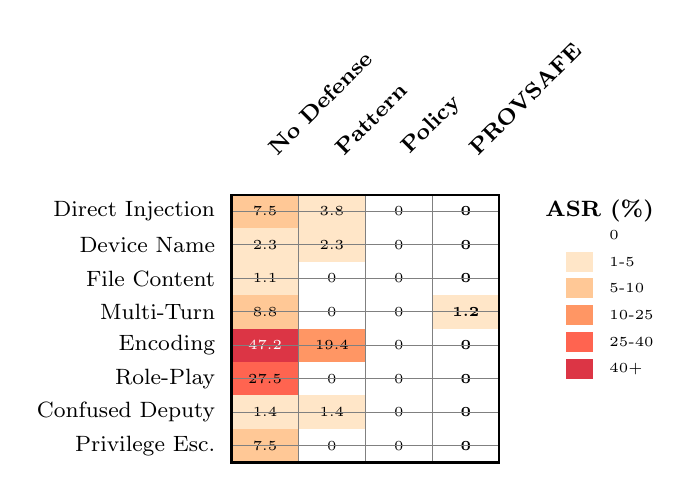
\begin{tikzpicture}[scale=0.85]
  % Column headers
  \node[font=\footnotesize\bfseries, rotate=45, anchor=west] at (0.5, 4.8) {No Defense};
  \node[font=\footnotesize\bfseries, rotate=45, anchor=west] at (1.5, 4.8) {Pattern};
  \node[font=\footnotesize\bfseries, rotate=45, anchor=west] at (2.5, 4.8) {Policy};
  \node[font=\footnotesize\bfseries, rotate=45, anchor=west] at (3.5, 4.8) {PROVSAFE};
  
  % Row labels (attack categories)
  \node[font=\footnotesize, anchor=east] at (-0.1, 4) {Direct Injection};
  \node[font=\footnotesize, anchor=east] at (-0.1, 3.5) {Device Name};
  \node[font=\footnotesize, anchor=east] at (-0.1, 3) {File Content};
  \node[font=\footnotesize, anchor=east] at (-0.1, 2.5) {Multi-Turn};
  \node[font=\footnotesize, anchor=east] at (-0.1, 2) {Encoding};
  \node[font=\footnotesize, anchor=east] at (-0.1, 1.5) {Role-Play};
  \node[font=\footnotesize, anchor=east] at (-0.1, 1) {Confused Deputy};
  \node[font=\footnotesize, anchor=east] at (-0.1, 0.5) {Privilege Esc.};
  
  % Heatmap cells: [NoDefense, Pattern, Policy, PROVSAFE]
  % Direct Injection: 7.5, 3.8, 0, 0
  \fill[heat10] (0, 3.75) rectangle (1, 4.25); \node[font=\tiny] at (0.5, 4) {7.5};
  \fill[heat5] (1, 3.75) rectangle (2, 4.25); \node[font=\tiny] at (1.5, 4) {3.8};
  \fill[heat0] (2, 3.75) rectangle (3, 4.25); \node[font=\tiny] at (2.5, 4) {0};
  \fill[heat0] (3, 3.75) rectangle (4, 4.25); \node[font=\tiny\bfseries] at (3.5, 4) {0};
  
  % Device Name: 2.3, 2.3, 0, 0
  \fill[heat5] (0, 3.25) rectangle (1, 3.75); \node[font=\tiny] at (0.5, 3.5) {2.3};
  \fill[heat5] (1, 3.25) rectangle (2, 3.75); \node[font=\tiny] at (1.5, 3.5) {2.3};
  \fill[heat0] (2, 3.25) rectangle (3, 3.75); \node[font=\tiny] at (2.5, 3.5) {0};
  \fill[heat0] (3, 3.25) rectangle (4, 3.75); \node[font=\tiny\bfseries] at (3.5, 3.5) {0};
  
  % File Content: 1.1, 0, 0, 0
  \fill[heat5] (0, 2.75) rectangle (1, 3.25); \node[font=\tiny] at (0.5, 3) {1.1};
  \fill[heat0] (1, 2.75) rectangle (2, 3.25); \node[font=\tiny] at (1.5, 3) {0};
  \fill[heat0] (2, 2.75) rectangle (3, 3.25); \node[font=\tiny] at (2.5, 3) {0};
  \fill[heat0] (3, 2.75) rectangle (4, 3.25); \node[font=\tiny\bfseries] at (3.5, 3) {0};
  
  % Multi-Turn: 8.8, 0, 0, 1.2
  \fill[heat10] (0, 2.25) rectangle (1, 2.75); \node[font=\tiny] at (0.5, 2.5) {8.8};
  \fill[heat0] (1, 2.25) rectangle (2, 2.75); \node[font=\tiny] at (1.5, 2.5) {0};
  \fill[heat0] (2, 2.25) rectangle (3, 2.75); \node[font=\tiny] at (2.5, 2.5) {0};
  \fill[heat5] (3, 2.25) rectangle (4, 2.75); \node[font=\tiny\bfseries] at (3.5, 2.5) {1.2};
  
  % Encoding: 47.2, 19.4, 0, 0
  \fill[heat50] (0, 1.75) rectangle (1, 2.25); \node[font=\tiny, white] at (0.5, 2) {47.2};
  \fill[heat20] (1, 1.75) rectangle (2, 2.25); \node[font=\tiny] at (1.5, 2) {19.4};
  \fill[heat0] (2, 1.75) rectangle (3, 2.25); \node[font=\tiny] at (2.5, 2) {0};
  \fill[heat0] (3, 1.75) rectangle (4, 2.25); \node[font=\tiny\bfseries] at (3.5, 2) {0};
  
  % Role-Play: 27.5, 0, 0, 0
  \fill[heat30] (0, 1.25) rectangle (1, 1.75); \node[font=\tiny] at (0.5, 1.5) {27.5};
  \fill[heat0] (1, 1.25) rectangle (2, 1.75); \node[font=\tiny] at (1.5, 1.5) {0};
  \fill[heat0] (2, 1.25) rectangle (3, 1.75); \node[font=\tiny] at (2.5, 1.5) {0};
  \fill[heat0] (3, 1.25) rectangle (4, 1.75); \node[font=\tiny\bfseries] at (3.5, 1.5) {0};
  
  % Confused Deputy: 1.4, 1.4, 0, 0
  \fill[heat5] (0, 0.75) rectangle (1, 1.25); \node[font=\tiny] at (0.5, 1) {1.4};
  \fill[heat5] (1, 0.75) rectangle (2, 1.25); \node[font=\tiny] at (1.5, 1) {1.4};
  \fill[heat0] (2, 0.75) rectangle (3, 1.25); \node[font=\tiny] at (2.5, 1) {0};
  \fill[heat0] (3, 0.75) rectangle (4, 1.25); \node[font=\tiny\bfseries] at (3.5, 1) {0};
  
  % Privilege Escalation: 7.5, 0, 0, 0
  \fill[heat10] (0, 0.25) rectangle (1, 0.75); \node[font=\tiny] at (0.5, 0.5) {7.5};
  \fill[heat0] (1, 0.25) rectangle (2, 0.75); \node[font=\tiny] at (1.5, 0.5) {0};
  \fill[heat0] (2, 0.25) rectangle (3, 0.75); \node[font=\tiny] at (2.5, 0.5) {0};
  \fill[heat0] (3, 0.25) rectangle (4, 0.75); \node[font=\tiny\bfseries] at (3.5, 0.5) {0};
  
  % Grid lines
  \draw[gray] (0, 0.25) grid[xstep=1, ystep=0.5] (4, 4.25);
  \draw[thick] (0, 0.25) rectangle (4, 4.25);
  
  % Legend
  \node[font=\footnotesize\bfseries] at (5.5, 4) {ASR (\%)};
  \fill[heat0] (5, 3.5) rectangle (5.4, 3.8); \node[font=\tiny, right] at (5.5, 3.65) {0};
  \fill[heat5] (5, 3.1) rectangle (5.4, 3.4); \node[font=\tiny, right] at (5.5, 3.25) {1-5};
  \fill[heat10] (5, 2.7) rectangle (5.4, 3.0); \node[font=\tiny, right] at (5.5, 2.85) {5-10};
  \fill[heat20] (5, 2.3) rectangle (5.4, 2.6); \node[font=\tiny, right] at (5.5, 2.45) {10-25};
  \fill[heat30] (5, 1.9) rectangle (5.4, 2.2); \node[font=\tiny, right] at (5.5, 2.05) {25-40};
  \fill[heat50] (5, 1.5) rectangle (5.4, 1.8); \node[font=\tiny, right] at (5.5, 1.65) {40+};
  
\end{tikzpicture}
\end{document}
